\chapter{Medotologia}\label{cap:CnptDsng}

\section{Escolha da frequência}\label{sec:esc_freq}
A frequência foi escolhida com base no regulamento da Anatel. O mesmo estabelece que equipamentos de radiocomunicação com faixas restritas de: 902-907,5; 915-928; 2400-2483,5; 5725-5850 MHz, assim para os cálculos iniciais foi escolhida uma frequência de 920MHz.

\section{Estudo do Obstáculo}\label{sec:est_obs}
O primeiro passado adotado foi a análise dos pontos, verificando se entre os dois existia algum obstáculo. Essa informação pode ser extraída dos mapas que foram fornecidos em anexo, como mostra a figura \ref{fig:obs_cam}.
\begin{figure}[h]
	\centering
	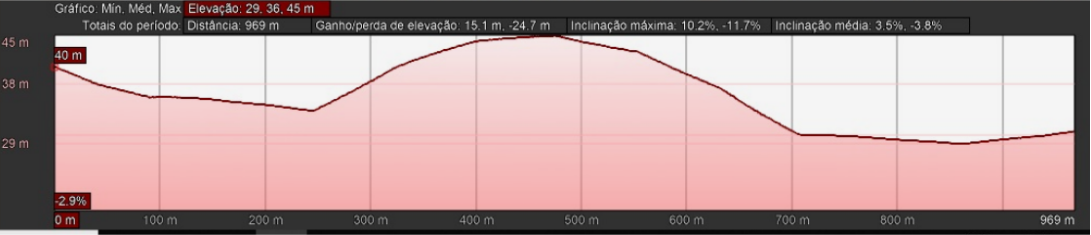
\includegraphics[width=1\textwidth]{obs_cam.png}
	\caption{Gráfico de obstáculo}
	\label{fig:obs_cam}
	%\source{Fornecido junto com os pontos}
\end{figure} 

Por meio da análise do gráfico, fica evidenciado que entre os dois pontos existe um grande obstáculo arredondado, assim sendo necessário calcular o seu raio de curvatura e a partir disso ver o quanto ele irá interferir na transmissão.
É feita uma aproximação do topo do obstáculo, utilizando uma curvatura parabólica como mostrado na figura 4 \ref{fig:obs_raio}.
\begin{figure}[h]
	\centering
	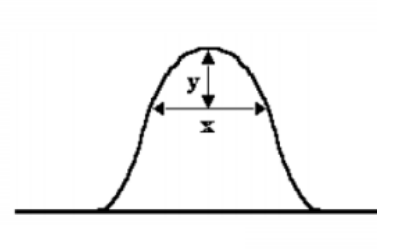
\includegraphics[width=.4\textwidth]{obs_raio.png}
	\label{fig:obs_raio}
	\caption{Curvatura parabólica utilizada para aproximação}
	%\source{Própria}
\end{figure} 

O raio $r$ da parábola será calculado o $\alpha$ que possibilita encontrar quantos decibéis de interferência o obstáculo irá causar. O cálculo do raio $r$ é feito utilizando a seguinte formula:
\begin{equation}
r = \dfrac{x^2}{8y}*10^{-3}
\end{equation}

Onde $x$ representa a distância em metros entre os dois pontos de igual nível, sendo um em cada lado do pico considerado e $y$ representa a diferença de cota entre o pico do obstáculo e a curva de nível considerada para  medida $x$.

\section{Atenuação do Obstáculo}
O cálculo do fator $\alpha$ relaciona a frequência $f$, o raio de curvatura da parábola $r$, a distância entre o vértice do obstáculo ao ponto de transmissão $d_1$ e a distância entre o vértice do obstáculo ao ponto de recepção $d_2$, ambas em \textit{Km}.
\begin{equation}
\alpha = 0,0818\dfrac{1}{\sqrt[6]{f}}\sqrt[3]{r}\sqrt{\dfrac{d_1+d_2}{d_1*d_2}}
\end{equation}

A atenuação é encontrada a partir de $\alpha$ e a relação entre os fatores  $H_c$ e $r_f$ por meio do gráfico 6. Onde $H_c$ representa a diferença entre ponto máximo do obstáculo e o nivelamento das antenas, enquanto $r_f$  é chamado de raio de \textit{fresnel}, sendo calculado com as mesmas distâncias $d_1$ e $d_2$. A relação é encontrada como mostrado na figura 6.

\begin{figure}[h]
	\centering
	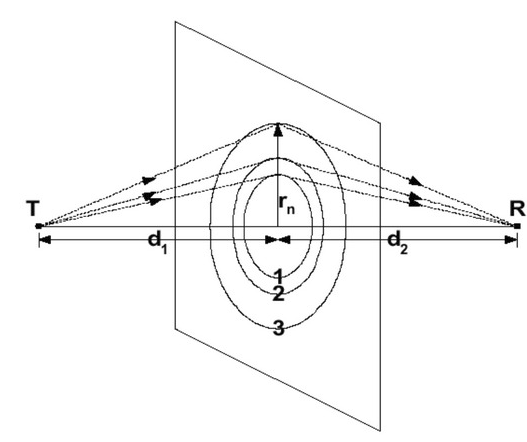
\includegraphics[width=.6\textwidth]{rf_img.png}
	\label{fig:rf_img}
	\caption{Modelo da zona de \textit{Fresnel}}
	%\source{Própria}
\end{figure}

O cálculo de $r_f$ se dá por:
\begin{equation}
r_f = \sqrt{\dfrac{n\lambda d_1 d_2}{d_1 + d_2}}
\end{equation}

\begin{figure}[h]
	\centering
	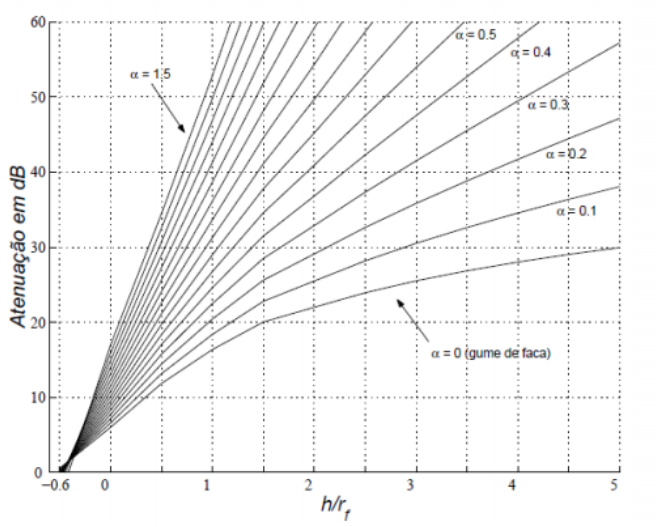
\includegraphics[width=.8\textwidth]{graf_ate.png}
	\label{fig:graf_ate}
	\caption{Gráfico de atenuação}
	%\source{Própria}
\end{figure} 


\begin{center}
	\begin{table}[]
		\begin{tabular}{|l|l|}
			\hline
			Rf    & 8,866 \\ \hline
			Hc    & 5     \\ \hline
			Hc/rf & 0,563 \\ \hline
		\end{tabular}
	\end{table}
\end{center}


\section{Atenuação no espaço livre}
O sinal também sofrerá atenuação ao ser transmitido no espaço livre, o cálculo da atenuação $L$ se dá por meio da fórmula de \textit{Fris}:
\begin{equation}
L = 32,45 +20(\log_{10}(d_1+d_2) + \log_{10}f)
\end{equation}



\section{Atenuação total}
A atenuação total é a soma da atenuação no espaço livre com a atenuação do obstáculo, assim :
\begin{equation}
L_{tot} = L + L_{obstaculo}
\end{equation}

\chapter{Resultados}
\section{Dados de entrada}
\subsection{Dados Gerais}
A altura escolhida para as torres foi de 0 e 9 para manter a linha de visada direta em paralelo com o chao e assim facilitando os cálculos e diminuindo os erros, os outros dados estão mostrados na tabela abaixo.
	\begin{table}[h]
		\centering
		\begin{tabular}{|
				>{\columncolor[HTML]{DAE8FC}}c |l|}
			\hline
			Distância Total (m) & 0,96713                  \\ \hline
			$\lambda$           & 0,001086957 x  $10^{-6}$ \\ \hline
			Altura das torres   & 0/9                      \\ \hline
		\end{tabular}
	\end{table}
\subsection{Dados dos Obstáculos}

\begin{table}[h]
	\centering
	\begin{tabular}{|
			>{\columncolor[HTML]{DAE8FC}}c |l|}
		\hline
		X                                                   & 325     \\ \hline
		Y                                                   & 7       \\ \hline
		$d_1$                                               & 0,475   \\ \hline
		\multicolumn{1}{|l|}{\cellcolor[HTML]{DAE8FC}$d_2$} & 0,49213 \\ \hline
	\end{tabular}
\end{table}
			
\section{Memorial de Cálculo}
\subsection{Frequência}
Não foi necessário calcular a frequência, o valor utilizado foi de 920MHz e sua escolha está justificada em \ref{sec:esc_freq}.

\subsection{Raio da Parábola}
Com os valores de $X$ e $Y$ do obstáculo o valor encontrado para o raio da parábola foi de:
\begin{equation}
	r_{parabola}= 1,886160714
\end{equation}

\subsection{Atenuação do obstáculo}
Com os valores de $d_1$ e $d_2$ o $\alpha$ encontrado teve valor de :
\begin{equation}
	\alpha = 0,6703932617
\end{equation}

O parâmetro $H_c$ foi encontrado por meio dos dados fornecidos, como mostrado na figura a seguir:
\begin{figure}[h]
	\centering
	\includegraphics[width=.8\textwidth]{hc.png}
	\label{fig:hc}
	\caption{Dados de $H_c$}
	%\source{Própria}
\end{figure} 

O parâmetro $r_f$ foi cálculado por meio da equação de $Fresnel$, com o valor dos parâmetros a seguir, foi encontrado no gráfico o valor da atenuação do obstáculo.

\begin{table}[h]
	\centering
	\begin{tabular}{|
			>{\columncolor[HTML]{DAE8FC}}c |l|}
		\hline
		$r_f$                                                         & 8,866    \\ \hline
		$H_c$                                                         & 5        \\ \hline
		$\dfrac{H_c}{r_f}$                                            & 0,563    \\ \hline
		\multicolumn{1}{|l|}{\cellcolor[HTML]{DAE8FC}$L_{obstaculo}$} & $22,5dB$ \\ \hline
	\end{tabular}
\end{table}

\subsection{Atenuação no Espaço livre}
Com os valores de $d_1$, $d_2$ e $f$ conhecidos o valor encontrado para $L$ foi:
\begin{equation}
L = 91,43dB
\end{equation}

\subsection{Atenuação total}
A atenuação total consiste nas soma das atenuação encontradas, logo:
\begin{equation}
L_{tot} = L + L_{obstaculo} = 91,43 + 22,5 = 113,9dB 
\end{equation} 

\section{Escolha do tranmissor e da antena}
 A escolha dos módulos e da antena se deu baseado na frequência escolhida para os cálculos e na versatilidade de cada dispositivo. 
 
 O modelo das antenas foi o \textit{Yagi(AirMax Antenna 900Mhz)},devido a sua faixa de trabalho e alta potência.
 
 O modelo do transmissor foi o \textit{Ubiquiti Networks(Rocket M9)} pot ser recomendado para trabalhar em conjunto com o modelo de antena \textit{Yagi}.
 \begin{figure}[h]
 	\centering
 	\includegraphics[width=.5\textwidth]{antena.jpeg}
 	\label{fig:antena}
 	\caption{Antena \textit{Yagi AirMax Antenna 900Mhz} }
 	\source{Ubiquiti Networks}
 \end{figure} 

\section{Receptor}
Escolha do receptor é encontrado à partir das potências das antenas, do módulo tranmissor e das perdas durante a transmissão. Sua potência foi calculada da seguinte forma:
\begin{equation}
	P_{receptor} = P_{antena_tx} + P_{antena_rx} + P_{transmissor} - L_{tot}
\end{equation}

A mesma antena utilizada para transmissão é utilizada para recepção, os dados da sua potência estão disponíveis nos seu \textit{datasheet} onde $P_{antena_{tx}} = P_{antena_{rx}} = 19dBi$. A potência do transmissõr também está disponível no datasheet, onde $P_{transmissor} = 28dBm$. O valor encontrado para potência do receptor foi de $	P_{receptor} = -47.9dBi$

Com o valor de $-47.9dBi$, o módulo \textit{Ubiquiti Networks(Rocket M9)} também poderá ser utilizado para recepção, tornando o sistema mais simplificado já que ambos receptores e transmissores estarão utilizando antenas recomendadas no datasheet.

\newpage
\begin{center}
	\Large \textbf{Variáveis do projeto}
\end{center}
Todos os valores utilizados e calculados estão registrados na figura a seguir:
\begin{figure}[h]
	\centering
	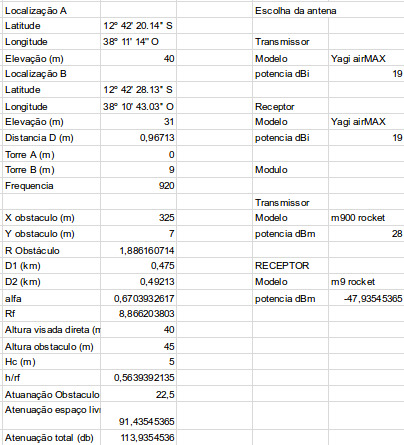
\includegraphics[width=1\textwidth]{resultados.jpeg}
	\label{fig:result}
	\caption{Variáveis do projeto}
	%\source{Própria}
\end{figure} 


